\documentclass[11pt, english]{article}
\usepackage{graphicx}
\usepackage[colorlinks=true, linkcolor=blue]{hyperref}
\usepackage[english]{babel}
\selectlanguage{english}
\usepackage[utf8]{inputenc}
\usepackage[svgnames]{xcolor}
\usepackage{url}
\usepackage{hyperref}
\usepackage{float}
\usepackage{longtable}
\usepackage[toc]{glossaries}

\usepackage{listings}
\usepackage{afterpage}
\pagestyle{plain}

\definecolor{dkgreen}{rgb}{0,0.6,0}
\definecolor{gray}{rgb}{0.5,0.5,0.5}
\definecolor{mauve}{rgb}{0.58,0,0.82}
\usepackage{biblatex}
\bibliography{ref.bib}

%\lstset{language=R,
%    basicstyle=\small\ttfamily,
%   stringstyle=\color{DarkGreen},
%    otherkeywords={0,1,2,3,4,5,6,7,8,9},
%    morekeywords={TRUE,FALSE},
%    deletekeywords={data,frame,length,as,character},
%    keywordstyle=\color{blue},
%    commentstyle=\color{DarkGreen},
%}

\lstset{frame=tb,
language=R,
aboveskip=3mm,
belowskip=3mm,
showstringspaces=false,
columns=flexible,
numbers=none,
keywordstyle=\color{blue},
numberstyle=\tiny\color{gray},
commentstyle=\color{dkgreen},
stringstyle=\color{mauve},
breaklines=true,
breakatwhitespace=true,
tabsize=3
}

\usepackage{here}


\textheight=21cm
\textwidth=17cm
%\topmargin=-1cm
\oddsidemargin=0cm
\parindent=0mm
\pagestyle{plain}

%%%%%%%%%%%%%%%%%%%%%%%%%%
% La siguiente instrucción pone el curso automáticamente%
%%%%%%%%%%%%%%%%%%%%%%%%%%

\usepackage{color}
\usepackage{ragged2e}

\global\let\date\relax
\newcounter{unomenos}
\setcounter{unomenos}{\number\year}
\addtocounter{unomenos}{-1}
\stepcounter{unomenos}
\gdef\@date{ Course \arabic{unomenos}/ 2019}

\makeglossaries
 


 
\newglossaryentry{igo}
{
    name=iGo,
    description={The online Ticket Vending Machine Web Application integrating with STM system}
}
\newglossaryentry{traveller}
{
    name=traveller,
    description={People who use STM metros and buses to travel daily in Montreal, Quebec, Canada}
}
\newglossaryentry{stm}
{
    name=STM,
    description={ Société de transport de Montréal (Montreal Transit Corporation)}
}
\newglossaryentry{opus}
{
    name=OPUS,
    description={OPUS is the name of STM travelling card which used by people to travel by STM services, manufactured and distributed by STM agencies}
}
\newglossaryentry{tvm}
{
    name=TVM,
    description={Ticket Vending Machine}
}
\newglossaryentry{cuigo}
{
    name=CUIGO,
    description={Context of use model for iGo}
}
\newglossaryentry{smigo}
{
    name=SMIGO,
    description={Stakeholder  Model representation for iGo}
}
\newglossaryentry{dmigo}
{
    name=DMIGO,
    description={Domain model representation for iGo}
}\newglossaryentry{ucmigo}
{
    name=UCMIGO,
    description={Use Case modelling for iGo}
}


\begin{document}

\begin{titlepage}

\begin{center}
\vspace*{-1in}
\begin{figure}[htb]
\begin{center}

\includegraphics[width=8cm]{logo}
\end{center}
\end{figure}
\begin{Large}
\textbf{SOEN 6481 - Software System Requirements Specification} \\
\end{Large}
\vspace*{0.1in}
Winter 2019\\
\vspace*{0.5in}
\begin{Large}
\textbf{Requirements Analysis for Ticket Vending Machine} \\
\end{Large}
\vspace*{0.4in}
\begin{large}
Project Report\\
\end{large}
\vspace*{0.2in}
\begin{Large}
\textbf{Deliverable 1} \\
\end{Large}
\vspace*{0.3in}
\begin{large}
Presented to \\
\vspace*{0.1in}
Instructor: PANKAJ KAMTHAN 
 \\
\end{large}
\vspace*{0.3in}
\rule{80mm}{0.1mm}\\
\vspace*{0.1in}
\begin{large}
By \\
Tran Minh Thy - 27131364\\
Suthakhar Ponnambalam - 40091123\\
Manasa Murali - 40082609\\
Prashanthi Ramesh - 40080517\\

\end{large}
\end{center}
\end{titlepage}

\newcommand{\CC}{C\nolinebreak\hspace{-.05em}\raisebox{.4ex}{\tiny\bf +}\nolinebreak\hspace{-.10em}\raisebox{.4ex}{\tiny\bf +}}
\def\CC{{C\nolinebreak[4]\hspace{-.05em}\raisebox{.4ex}{\tiny\bf ++}}}

\tableofcontents
\newpage
\section{Introduction}
This document provides an understanding of \gls{igo}, a ticket vending machine (TVM) which shall be used in Canada, Montreal, Quebec. 
\subsection{Purpose}
The purpose of this document is to collect, analyse and define needs and features of an online Ticket Vending Machine system (iGo) in Montreal, Quebec, Canada. It focuses on the features expressed by stakeholders which they would like to see in their application. This document provides details of how iGo - an online ticket vending machine fulfills these needs.It  describes the problems graphically with the context of use modeling, problem domain modeling, stakeholders modeling and use case modeling for different perspectives.
\subsection{Scope}
This document applies to the Online Ticket Vending Machine (called iGo)  in Montreal, Quebec, Canada, mainly for metros and buses. iGo plays as an online platform  allowing  travellers  to top up their \gls{opus} cards and manage \gls{stm} transactions themselves. iGo does not include the development and maintenance part of STM system and physical STM Ticket Vending Machines in STM offices.


\section{Product Overview}
\subsection{Problem Statement}
The majority of  transportation  we use daily in Montreal, Quebec, Canada is provided by STM (Montreal Transit Corporation) with buses and metros. People who travel via STM public transportation must use OPUS travelling card manufactured and distributed by STM. People must top up their OPUS card balance at the beginning of every month via physical STM Ticket Vending Machines (TVM) placed in STM stations. In order to top up their OPUS card, people often wait for a long queue in front of \gls{tvm} machines and STM office stations. The travelling process could be interrupted due to the fact that people usually forget to top up their OPUS card on time. \\ \\
iGo is an online Ticket Vending Machine Web Application that integrates with STM system allowing people do STM transactions online. People can connect and top up their OPUS cards online using their desktops or mobile devices at home. 

\subsection{iGo Description}
The solution designed to be an online web application allowing a \gls{traveller} to sign up, login, link and top up their OPUS cards. iGo will communicate with STM system over an appropriate communication link. \\

% \begin{table}[h]
%   \begin{center}
%     \label{tab:table1}
%     \begin{tabular}{|c|c|c|c|c|c|c|c|c|} 
%     \hline
%       $\alpha$ & Amparo & Borja & Daniel & Emilio & Jose & Maria Jesús & Raquel & Virginia\\
%       \hline
%      0.5  & 21461 & 21453 & 21412 & 21684 & 21503 & 21513 & 21676 & 21426\\ \hline
%      0.6 & 21553 & 21481 & 21406 & 21684 & 21487 & 21677 & 21685 & 21750\\ \hline
%      0.7 & 21793 & 21660 & 21697 & 21684 & 21577 & 21783 & 21818 & 21518\\ \hline
%      0.8 & 21783 & 21816 & 21735 & 21942 & 21952 & 21885 & 21884 & 21730\\ \hline
%      0.9 & 22080 & 22118 & 21895 & 22045 & 21951 & 22035 & 22008 & 21910\\
% \hline
%     \end{tabular}
%     \caption{2 minutes for each example to get our $\alpha$}
%   \end{center}
% \end{table}

A customer will be required to sign up an account with iGo on their first time. In order to top up or make transactions, a traveller is required to link their OPUS card number (displaying on their OPUS card)  with their iGo account. After signing up successfully, a traveller will be able to proceed one or more transactions. Their OPUS card will be linked to their iGo account and hence will be linked to all transactions that made under their iGo account. A traveller will be able to use their existing OPUS cards to travel in Montreal (Quebec, Canada) via buses and metros operated by STM. \\

\begin{figure}[h!]
  
  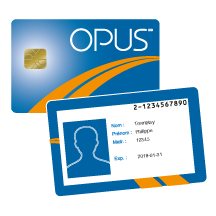
\includegraphics[width=0.5\textwidth]{opus.png}
  \centering
  \caption{Sample of OPUS card with the unique card number displaying on the back side, provided by STM (Montreal, Quebec, Canada)\cite{carte_opus}
}
\end{figure}

iGo must be able to provide the following services to Montreal travellers:
\begin{enumerate}
  \item A traveller must be able to sign up to an iGo account online, with their email address and be able to link their OPUS card number to their iGo account.
  \item A traveller must be able to make a payment transaction to an OPUS card that is linked to their iGo account. After login, a traveller will enter the amount to make a payment. The transaction could be made via Visa or Mastercard, or Paypal. 
  \item A traveller must be able to view their existing OPUS card balance. 
  \item A traveller must be able to view their OPUS transactions, and must be able to print out their transactions.
  \item A traveller must be able to add multiple OPUS cards under one iGo account.
  \item A traveller must be able to schedule their payments for their OPUS card. 
  \item A traveller must be able to use their OPUS card to go through buses or metroes. The OPUS scanner at STM gates and STM buses must be able to detect if the OPUS card has a sufficient balance.
  \item A traveller must be able to un-link any OPUS cards under their iGo account.
  
\end{enumerate}
iGo will communicate each transaction to STM System and obtain the verification that was allowed by STM. Ordinally, a transaction will be considered complete by STM once it has been paid successfully and it has been approved by STM. iGo will connect with STM System to make sure transactions are successfully made.\\

If  STM determines that the email exists in STM database, a traveller will be required to login or use another email to register. If STM determines that the STM card number is linked to another existing iGo account, a traveller will not be able to link this OPUS card number to their iGo account unless that iGo account unlinks this OPUS card on iGo. In all cases, iGo is required to display an explanation of the problem. \\

iGo will also maintain its internal log of transactions to facilitate resolving ambiguities arising from a connection failure in the middle of transactions between iGo and STM System. Entries will be made in the log when a traveller registers an account, logs in and  working on their their login session. \\

\begin{figure}[H]
  
  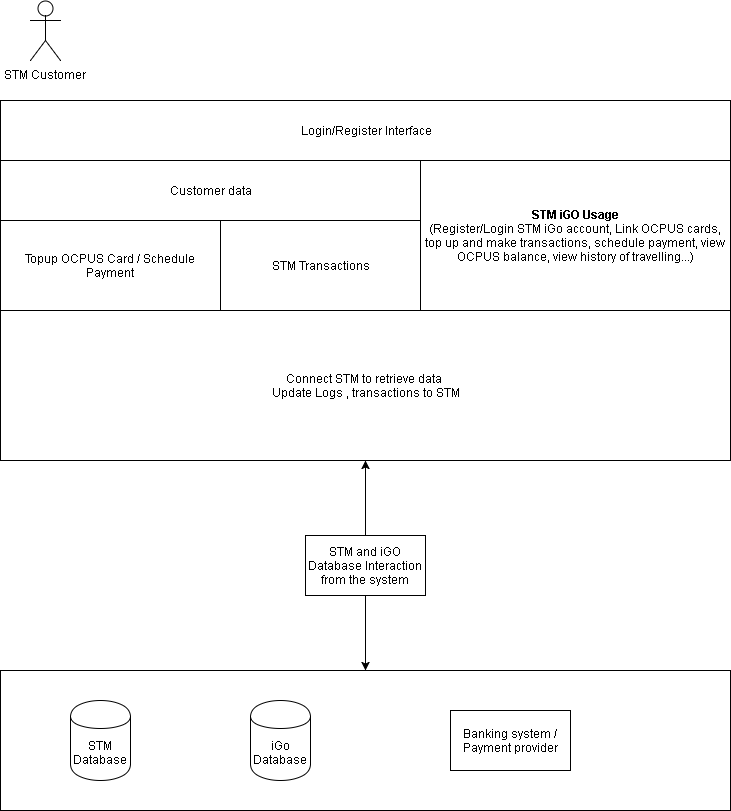
\includegraphics[width=0.8\textwidth]{ContextOfUse.png}
  \centering
  \caption{ Overview of the STM iGo architecture}

\end{figure}

\subsubsection{Project Assumption}

For this project, iGo does not implement STM Card Readers which will be installed on buses and metros entries. Assumption is made that STM will implement and install STM Card Readers which will be able to detect a STM card by its number, checking its balance and updating it in STM’s system.

\section{Context of Use}

We use the user-centric context of use framework \cite{contextofusecasekamthan}  to identify and classify factors that influence the utility and usability of iGo.\\



\setlength{\tabcolsep}{18pt}
\renewcommand{\arraystretch}{1.5}
\begin{tabular}[H]{ |p{3cm}|p{12cm}| }
\hline
Factor   & Description  \\
\hline
User &   \\
\hline
Experience & 
Users who daily transit with STM metros and buses will have their daily OPUS cards to be able to link with iGo. These users have experiences in using OPUS cards, therefore they understand how STM and iGo work easier. (such as what is STM, what is OPUS card, how much payment to top up OPUS…)
Users who have experiences on online transactions (example: online shopping) will find it easier to understand to apply their experience to use iGo.
Users who do not have any experiences on online transactions, who never use computers, who never use mobile devices, will find it complicated to use iGo, and therefore, they may not use iGo.
    \\
\hline
Education &
Users who are not able to read in English or French, will not be able to use iGo web system.
Users who are not computer-aware will not be able to use iGo web system.
 \\
 \hline
Physical Characteristics    &
Users who are blind will not be able to use iGo web system because iGo does not support text-reading feature.
  \\
  \hline
Cognitive Characteristics & 
Users who are familiarised in online transactions will be able to use iGo quickly.
  \\
 \hline
Task &  \\
\hline
Complexity & 
The complexity of iGo web application will affect the usage experiences of users. The higher complexity of iGo web application is, the higher in usage resistance will be.
  \\
\hline
Demands &

The demands of iGo web application is high due to the fact that:
\begin{enumerate}
    \item Long queue and inconvenience that travellers must face when they top up their OPUS cards using STM physical Ticket Vending Machines.
    \item Montreal city is one of top 3 high-tech cities in Canada and one of 25 high-tech cities in the world. iGo suites the demand of people who want to enjoy the convenience of technology in their STM daily transit.\cite{tech_city}
\end{enumerate} \\
\hline 
\end{tabular}
\\ 


\setlength{\tabcolsep}{18pt}
\renewcommand{\arraystretch}{1.5}
\begin{tabular}{ |p{3cm}|p{12cm}| }
\hline
Workflow Controllability & The workflow of iGo web application should be simple for users to understand. Target end users could be senior citizens or young children who are expected to use iGo efficiently.\\
\hline
Safety & 
iGo is an online web application which will not cause any damage or injuries to travellers. The safety of using iGo is high which is a positive.\\
\hline
Criticality & 
iGo is expected to work accurately. Travellers who choose iGo to top up and manage their OPUS transactions are able to use OPUS on all STM metros and buses. Any errors caused during online transaction processes are not accepted.\\
\hline
Environment & \\
\hline
Physical Environment & 
In order to use iGo, travellers are expected to have a computer or mobile device connecting to the Internet. Devices are expected to support web browsing.\\
\hline
\end{tabular}
\vspace*{0.3in}
The above table describes the \gls{cuigo} of iGo\\
\section{Stakeholders and Users Description}
\subsection{Stakeholders mind map}

\begin{figure}[H]
  
  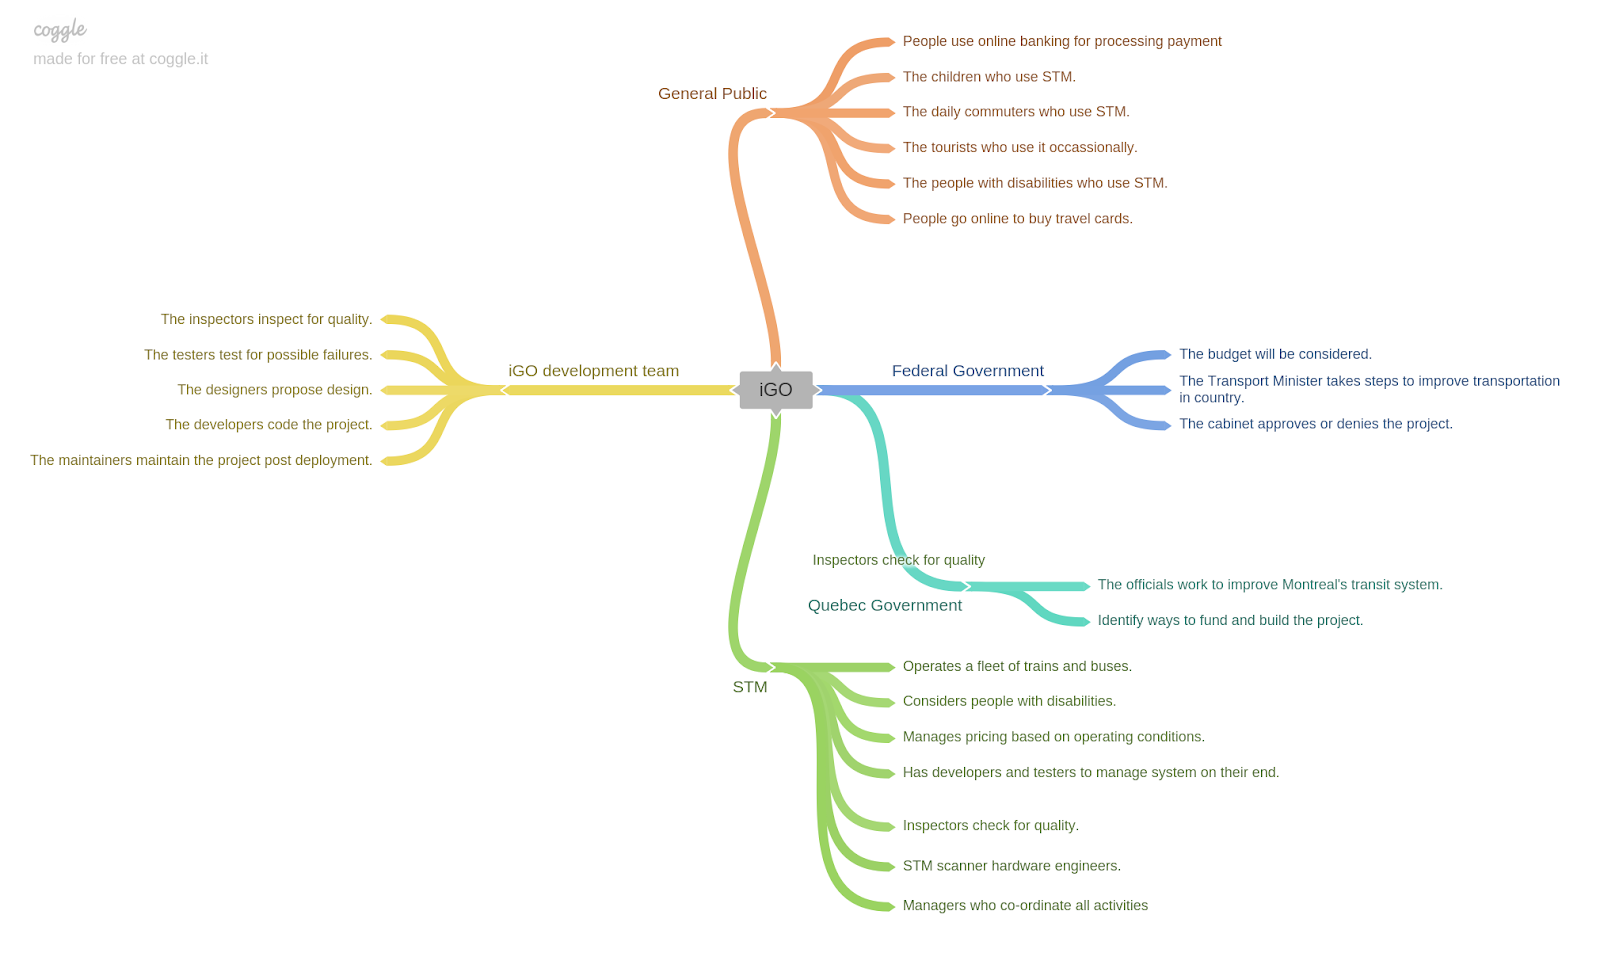
\includegraphics[width=0.8\textwidth]{iGO_stake.png}
  \centering
  \caption{The mindmap model (\gls{smigo}) depicting the functions of every team involved in iGO}
  \end{figure}
  Due to the context of use of iGo, a stakeholder mind map has five main branches:
  \begin{enumerate}
      \item iGo Development team 
\item STM 
\item Federal Government
\item Quebec Government
\item General Public who are travelling via STM transportation in Quebec’s Montreal city. 

  \end{enumerate}


iGo development team and STM are two main stakeholder groups without whom iGo project could not succeed. Since iGo and STM are related to a public transportation that operates daily transit services in Montreal, Quebec, Canada, two other stakeholders group must be analysed, which are the Federal Government of Canada and the Quebec Government. The last stakeholder group that directly uses and enjoys benefits of iGo - Montreal city residents must also be analysed. 

\subsection{Stakeholders description}
After discovering stakeholders via mind mapping method, we come up with two main group of stakeholders:
\begin{enumerate}
    \item Non-User stakeholders: Stakeholders who are not end users of an iGo system. They may be affected by the influence of iGo (positively or negatively) or they may affect the success of iGo. We group them into Non-User stakeholders group.
    \item End-User stakeholders:
Stakeholders who are end users of an iGo system, who directly benefit from iGo features and who directly interact with iGo system.

\end{enumerate}

\subsubsection{Non-user stakeholders}
\vspace*{0.1in}
\setlength{\tabcolsep}{18pt}
\renewcommand{\arraystretch}{1.5}
\begin{tabular}{ |p{3cm}|p{7cm}|p{3cm}| }
\hline
Name & Description & Responsibilites\\
\hline

Quebec Government &
This is a stakeholder who must give permissions to let iGo and STM integrate. &
Support STM and iGo in the law perspectives.\\
\hline
Federal Government of Canada and Transport Minister of Canada &
This is a stakeholder who must give permissions to let iGo and STM integrate. This stakeholder group has the same authority level with Quebec Government in this project. &
Support STM and iGo in the law perspective.\\
\hline
\end{tabular}
\pagebreak

\setlength{\tabcolsep}{18pt}
\renewcommand{\arraystretch}{1.5}
\begin{tabular}{ |p{3cm}|p{7cm}|p{3cm}| }
\hline
STM Office Management &
This is a stakeholder who provides the business logic and management support for iGo development team. &
Verify iGo business requirements. 
Inform existing customers about iGo 
Support customers during the transition from STM TVM to iGo. \\
\hline
iGo Developers & 

This is a stakeholder who must be involved regularly to maintain  the development cycle of iGo. &
Develop iGo according to verified business requirements.\\
\hline
iGo Business Analyst &
This is a stakeholder that works with Analysts in STM to correctly translate requests or needs into requirements to be used for development. &
Specifies details of iGo’s functionalities.\\
\hline

iGo Project Manager &
This is a stakeholder who is leading iGo system development. &
Acts as an intermediary between the development team and the STM. Responsible for tracking the status of the project within budget and schedule\\
\hline
STM Developers &
This is a stakeholder who must be involved regularly to maintain  the development cycle of iGo. &
Develop iGo REST APIs to connect to STM internal system. \\
\hline
STM Business Analyst &
This is a stakeholder that works with analysts in iGo to correctly translate requests or needs into requirements to be used for development. &
Specifies details of iGo’s functionalities to be compatible with STM.\\
\hline
\end{tabular}
\pagebreak

\setlength{\tabcolsep}{18pt}
\renewcommand{\arraystretch}{1.5}
\begin{tabular}{ |p{3cm}|p{7cm}|p{3cm}| }
\hline
STM Project Manager &
This is a stakeholder who is leading for iGo and STM integration system development. &
Acts as an intermediary between STM authorities and the iGO software management team.\\
\hline
Local business who do the top up services for STM card &
 Local businesses have an STM top up charger which allows people to top up their OPUS cards without visiting TVM machine in STM offices. This stakeholders will not be happy with iGo success because they will lose their revenue. \cite{opus_card_at_home}&


Not applicable\\
\hline

\end{tabular}

\subsubsection{User stakeholders}
\vspace*{0.1in}
\setlength{\tabcolsep}{18pt}
\renewcommand{\arraystretch}{1.5}
\begin{tabular}{ |p{3cm}|p{4cm}|p{6cm}| }
\hline
Name & Description & Responsibilities\\
\hline

Customers who have STM cards &
Primary end users of iGo &
Use iGo online web application for topping up their OPUS cards and managing their STM transactions. \\

\hline

\end{tabular}

\subsection{Stakeholders model}
After analysing responsibilities of stakeholders , we come up with the following stakeholder model, describing their influence to iGo. The further the stakeholders from iGo, the least influence level that they may bring to iGo.

\begin{figure}[H]
  
  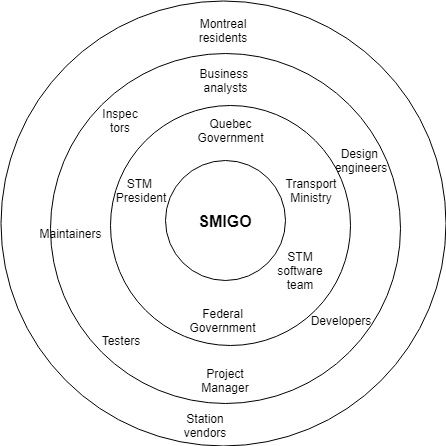
\includegraphics[width=0.8\textwidth]{onion.png}
  \centering
  \caption{ The Onion model representation for IGO (SMIGO)}

\end{figure}
We prioritise  iGo stakeholders  based on their influence and importance in a sense that without them, iGo shall fail.
\\
 \begin{itemize}
   \item  Critical
   \begin{itemize}
     \item  The Federal and Quebec Governments has the highest priority because they shall give permissions on iGo’s connection to STM Cloud as well as finance for iGo.
    \item The iGO development team and STM development team has an equal influence because they develop and maintain iGo system.\\ \\ \\
   \end{itemize}
   \item  Major
   \begin{itemize}
     \item  The STM representatives in the major list as they plan and verify the needs of the customers and its employees.
\item Montreal citizens are major stakeholders because they are direct users of the system. Their feedbacks and their needs are important to the success of iGo.

   \end{itemize}
    \item  Minor
   \begin{itemize}
     \item Local businesses who service customers to top up OPUS cards via their OPUS scanners are the least influence stakeholders. They have no responsibilities and less to say about iGO.

   \end{itemize}
 \end{itemize}
 
 \begin{figure}[H]
  
  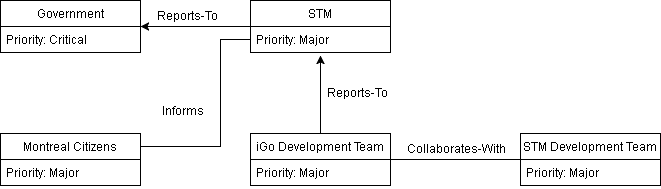
\includegraphics[width=0.8\textwidth]{StakeholderRelationship.png}
  \centering
  \caption{ Stakeholders relationship model}

\end{figure}

\section{Problem Domain}
\subsection{Problem Domain Model}

 \begin{figure}[H]
  
  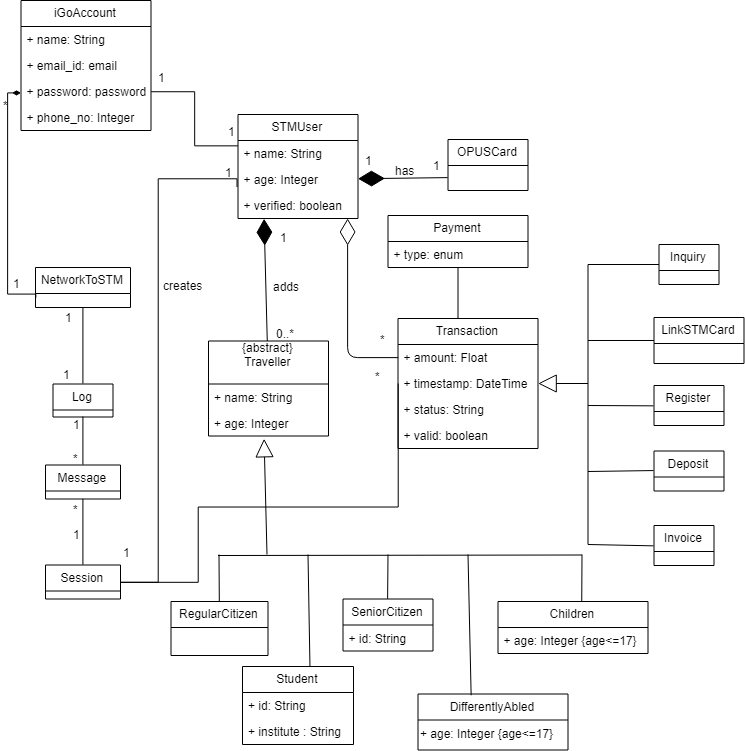
\includegraphics[width=0.8\textwidth]{domain_model_final.png}
  \centering
  \caption{Domain Model of IGo (\gls{dmigo})}

\end{figure}

The domain model\cite{domainkamthan} of our iGo system is represented by several classes. The purpose of the diagram is to show and explain our iGo system, the travellers (senior citizens, regular citizens, children, students and differently abled), their relationships with the STM system and the banking system in terms of payment. \\



They all have some common characteristics such as name or age, and they use STM services, so in our problem domain model, these entities are inherited from the abstract class Traveller. Also, not all travellers may have OPUS cards because some of them are paying cash per usage. Therefore, User entity includes STM users who have at least one OPUS card to travel daily with STM services.\\

The STM users can create an iGo account , which is represented as an account entity. One STM user can have only one OPUS card, whereas, a single iGo account can have many users in their account. Our system is unique in its sense that a family can have one iGo account and add many travellers and link many OPUS cards. \\

The traveller can make a payment for his/her transaction and can do it either through mastercard, visa card or PayPal. The banking system will authorise this transaction and on successful payment, the customer can view their transaction details and even print the same. But, not all travellers may have OPUS cards because some of them are paying cash per usage. Therefore, User entity includes STM users who have at least one OPUS card to travel daily with STM services.(
The customer can also schedule their payments and pre authorise the payment by filling in their card details and the bank will also validate the card on this. \\

\section{Use Case Model }
\subsection{Use Case Diagram}
 \begin{figure}[H]
  
  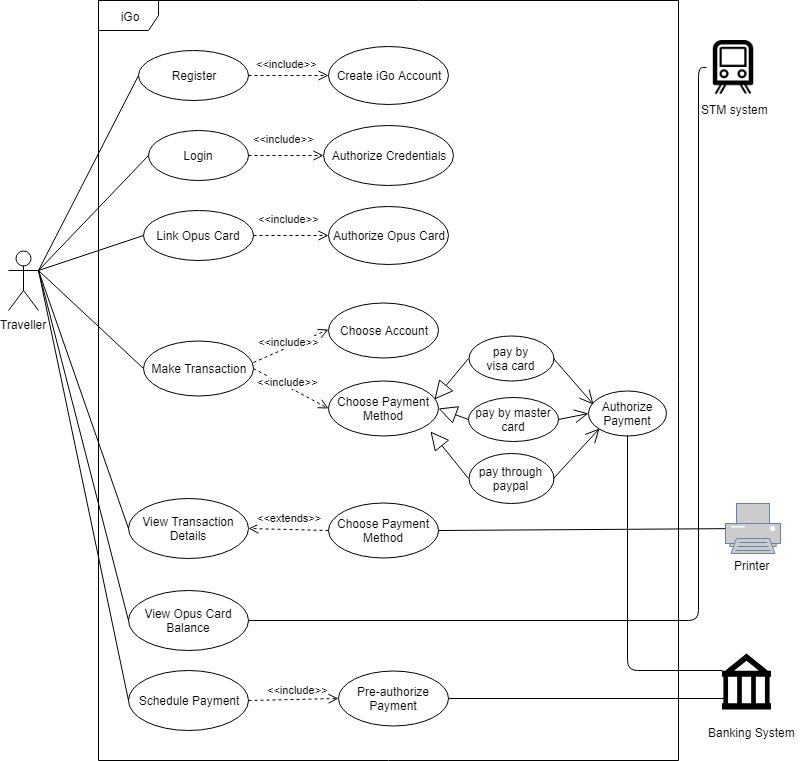
\includegraphics[width=0.8\textwidth]{usecase_model.png}
  \centering
  \caption{Use case model of iGo System (\gls{ucmigo})}

\end{figure}

 \begin{figure}[H]
  
  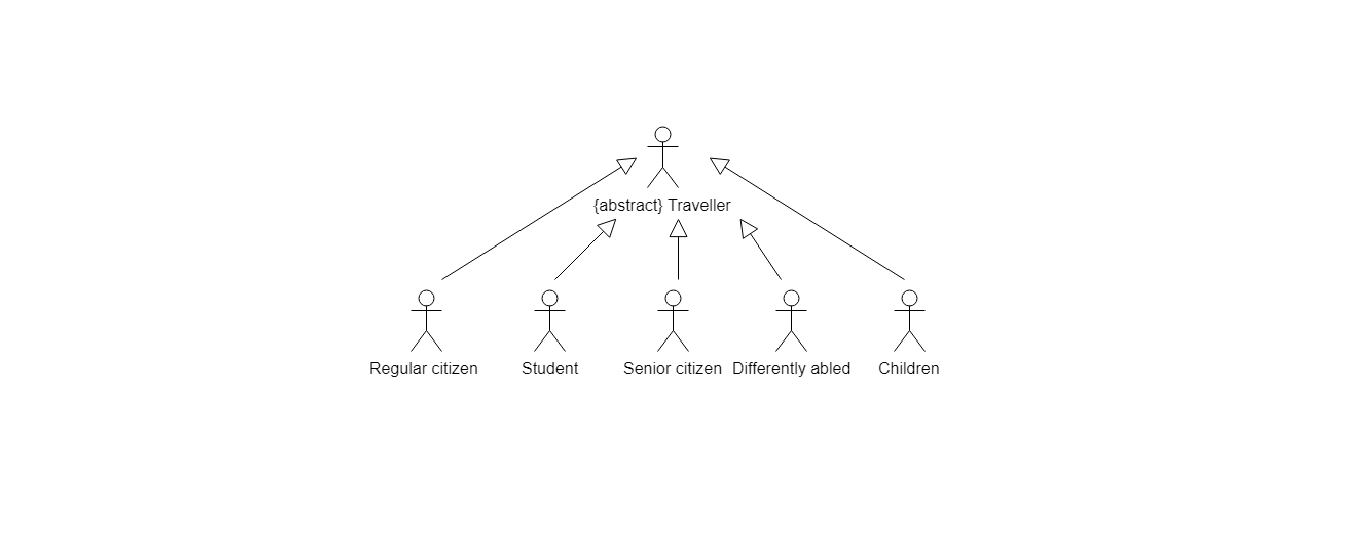
\includegraphics[width=0.8\textwidth]{final.png}
  \centering
  \caption{Types of Actors in iGo}

\end{figure}

\subsection{Use Case Brief}

Register an iGo account\\
Actor: STM customers\\
A STM customer needs to register to an iGo account with his email address. iGo will authenticate a user with STM system via REST APIs developed by STM developers. iGo will display error or successful message returned by STM.\\ \\
 Login in iGo\\
Actor: iGo user, STM System \\
iGo users login to the iGo website using his/her credentials. STM system authorises iGo user’s credentials.\\ \\
Link OPUS card to iGo account \\
Actor: iGo user, STM System\\
iGo users try to link their OPUS card with STM system. STM system must validate and link OPUS card to STM account using OPUS card number which is unique for each card. iGo must be able to display success or failure message to users based on response from STM system.\\ \\
 Make Transaction \\
Actor: iGo user, STM System, Bank\\
iGo user makes a payment either by using Visa, Mastercard or Paypal. iGo will connect the payment with Banks. Banks must authorise and respond the payment status to iGo. If the payment status is successful, iGo will send the transaction data to STM system. \\ \\
View Transaction Details \\
Actor: iGo user, STM System\\
The user can view his/her transaction history via iGo by selecting a linked OPUS card. STM system must return transaction history to display to an iGo user. \\ \\
View OPUS Card Balance\\
Actor: iGo user, STM system \\
iGo users can check their OPUS balance. iGo will send the request to STM system via REST APIs. STM system must be able to return corresponding data related to selected card’s OPUS balance.\\ \\
 Schedule Payment\\
Actor: iGo user, Bank\\
iGo user can schedule their advance payments for their selected OPUS cards. iGo will send a request to the bank. The bank must be able to authorise the payment and return the success or failure response message to iGo. If the status is successful, iGo will handle the schedule payment.\\ \\

 \begin{figure}[H]
  
  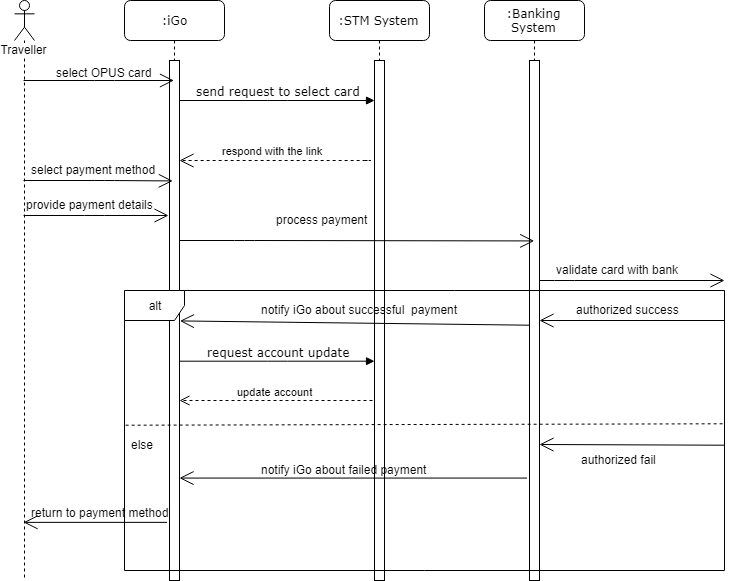
\includegraphics[width=0.8\textwidth]{seqfinal1.png}
  \centering
  \caption{Sequence Diagram depicting the scenario of the Make Payment use case}

\end{figure}

The above diagram shows the sequence diagram for the Make Payment use case 
It shows the sequence in which the flow goes with the involvement of actor (Traveller), iGo, STM System and the Bank. The payment can either be successful or failed. For a successful payment, the iGo gets notified about the same and asks the STM  system to update the account otherwise the failed payment error leads to the previous select payment method page. 

\section{Conclusion}
The document goes through problems that existing STM travellers may face with the traditional method of topping OPUS card via STM physical Ticket Vending Machines. The document introduces the concept of iGo (an online web application to provide an alternative solution for STM physical TVM) expressively via Context of Use Model, Stakeholders models, Domain Problem Model and Use Case Model. 


\printbibliography

\printglossary

\end{document}